% contributed by Ulrike Fischer
\documentclass{standalone}
\usepackage{tikzducks}
\pagecolor{gray!20!white}
\begin{document}
	
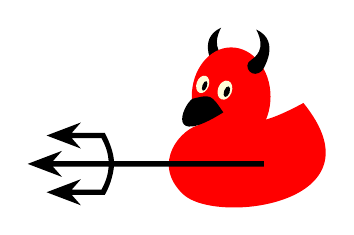
\begin{tikzpicture}
	\duck[
		grumpy,
		body=red,
		devil=black,
		bill=black,
		grumpy
	]
	\begin{scope}[yshift=-1.3cm,xshift=-1.8cm,scale=0.9]
		\fill (0.8800,1.5776) -- (0.4879,1.7266) -- (0.3956,1.7618) -- (0.8800,1.9458) -- (0.7507,1.7993) -- (1.1706,1.7993) .. controls (1.2317,1.9102) and (1.2653,2.0175) .. (1.2717,2.1245) -- (0.4838,2.1245) -- (0.6132,1.9780) -- (0.2210,2.1270) -- (0.1287,2.1620) -- (0.6132,2.3462) -- (0.4838,2.1995) -- (1.2717,2.1995) .. controls (1.2653,2.3065) and (1.2317,2.4139) .. (1.1706,2.5247) -- (0.7507,2.5247) -- (0.8800,2.3782) -- (0.4879,2.5272) -- (0.3956,2.5622) -- (0.8800,2.7464) -- (0.7507,2.5997) -- (1.2165,2.5997) .. controls (1.2844,2.4710) and (1.3392,2.3246) .. (1.3469,2.1995) -- (3.4630,2.1995) -- (3.4630,2.1245) -- (1.3469,2.1245) .. controls (1.3275,1.9688) and (1.2818,1.8391) .. (1.2165,1.7243) -- (0.7507,1.7243) -- cycle;
	\end{scope}	
\end{tikzpicture}	
	
\end{document}